\documentclass[a4paper,12pt, oneside]{book}
\usepackage{graphicx}
\usepackage{natbib}
\usepackage{float}
\usepackage{lettrine}
\usepackage{hyperref}
\usepackage{minted}
\usepackage{fontspec}
\setmainfont{EB Garamond}
\setmonofont{inconsolata}
\graphicspath{{./image/}}
\linespread{1.25}
\title{Very Naive MIPS CPU using Clash}
\author{ZHU Yifan (118010469) <i@zhuyi.fan>}
\begin{document}
\frontmatter
\maketitle
\chapter*{}
\vspace*{\fill}
In memory of Carl Quinn, for his great contributions to the field of Programming Languages.
\begin{figure}[H]
	\centering
	
\includegraphics[scale=0.8]{cquinn}
\end{figure}
\vspace*{\fill}
\chapter{Introduction}
In CUHK(SZ) and many other universities, writing an MIPS CPU with pipeline is a required work for the  architecture courses. However, most teaching materials just provide students with some basic concepts of CPUs and do not give essential introductions on languages or the potential difficulties of the implementation.
Writing this book, we want to achieve the following goals:
\begin{itemize}
	\item Give a detailed description on each part of the MIPS CPU.
	\item Clarify how we can write a sequential logic circuit, avoiding oscillations and other problems.  
	\item Introduce Clash, a higher level HDL that can generate synthesizable Verilog files and reduce the complexity of development. 
\end{itemize} 

We are \textbf{NOT} going to implement a fully functional MIPS CPU. Instead, we will only structure some skeletons that can help us understand the concepts and principles. We hope the readers can gain some basic knowledge of hardware design and the Clash language from this book.

\tableofcontents

\mainmatter
\chapter{Preparation}
\lettrine{R}{ight} before our journey of implementing the MIPS CPU using Clash language, we need to get our equipment ready.
\section{Prerequisites of this Book}
Reading this book, you are expected to have some basic knowledge of Verilog HDL and the Haskell language. However, if you happen to have little experience on these two languages, do not worry too much; they are just the language tools that we are going to use to express the logic and thoughts. The expressions should be easy to understand and we are going to provide some detailed descriptions on those critical lines.   

It is also a good idea to acquire some basic knowledge about Digital Logic Circuits. You'd better grab the concepts of clock, combinatorial logic and sequential logic.
\section{Install iVerilog}
iVerilog is a tool to synthesis Verilog sources and generate simulation executables. We are going to use it as our default Verilog compiler. It is available to GNU/Linux, Mac OS and Windows.

Windows users can follow \href{http://bleyer.org/icarus/}{this link} (\mintinline{text}{http://bleyer.org/icarus/}) to download it.

Mac users can follow \href{https://blog.csdn.net/zach_z/article/details/78787509}{this tutorial}

(\mintinline{text}{https://blog.csdn.net/zach_z/article/details/78787509}) to download it.

As for GNU/Linux users, I believe you have already found a way to get it work.

\section{Prepare Haskell Environment}
We are using stack for the projects. It should be easy to install, just go through \href{https://docs.haskellstack.org}{this document} (\mintinline{text}{https://docs.haskellstack.org}) to get all the requirements settled. 

As for Clash, there are several ways to install it. It is ready for Nix build system, Snapcraft and it is also doable to compile it from the source. You are recommended to visit \href{https://clash-lang.org}{its website} (\mintinline{text}{https://clash-lang.org}) before you start installing it.

After all things are settled, you should be able to play with the template project at GitHub, under dramforever/clash-with-stack (Great thanks for \textbf{dramforever}).

Its clash version is a little bit old, but it is enough for this book. Feel free to upgrade the version to the latest ones (tested until 1.2.0).

This template does not use \mintinline{yaml}{mtl} library that we needs (for the state monad), you may need to add it on you own at the \mintinline{text}{package.yaml}.
\chapter{Essential Verilog}
\lettrine{W}{e} would like to introduce some basic Verilog knowledge that will be used in this book. We will not go into details here, just showing some most common use cases. Let us first take a look at the final outcome of our project.
\section{Module Interface}
\begin{minted}[linenos, breaklines]{verilog}
`timescale 100fs/100fs
module CPU 
    ( input  CLOCK // clock
    , input  RESET // reset
    , input  ENABLE
    );
    wire [32:0] BRANCH;
    wire [30:0] PC_INSTRUCTION;
    wire [31:0] PC_VALUE;
    wire [37:0] WRITE_PAIR;
    wire        STALL;
    wire [5:0]  DM_WRITE;
    wire [1:0]  DM_MEM;
    //...

    InstructionModule IM
    ( // Inputs
    .CLOCK(CLOCK), // clock
    .RESET(RESET), // reset
    .ENABLE(ENABLE),
    .BRANCH(BRANCH),
    .STALL(STALL),

    // Outputs
    .PC_INSTRUCTION(PC_INSTRUCTION),
    .PC_VALUE(PC_VALUE)
    );
    // ...

    assign AM_FW_0 = MMO_WRITE_PAIR;

    assign AM_FW_1 = WB_WRITE_PAIR;

    assign WRITE_PAIR = WB_WRITE_PAIR;

    assign BRANCH  = WB_BRANCH;
    
endmodule
\end{minted}
These lines are extracted from the CPU source code. 
\begin{enumerate}
	\item The first line is a compiler derivative that defines the precision of timing;
	\item Line 2 to line 6 define the module interface of a CPU, with three input ports. As for outputs, you can add something like \mintinline{verilog}{output wire OUTPUT};
	\item Line 7 to line 13 declare some wire variables. As you can see, you can point out the number of bits in the declaration. Wires are used to connect different components of the circuits, you can treat them as a renaming of the original port because the value of a wire is refreshed as soon as the input side changes.
	\item Apart from wires, another commonly used thing is \mintinline{verilog}{reg [31:0] REGISTER}; you can treat this as the variables in the common sense, which has its own state.
	\item \mintinline{verilog}{InstructionModule IM (...)} declares a component named \mintinline{verilog}{IM} whose definition is in another module called \mintinline{verilog}{InstructionModule};
	\item There are mainly two ways to interact with another module, one is to use it as what is listed in the code: use a syntax like \mintinline{verilog}{.PORT(SOME_WIRE)} to connect the inputs and outputs; the other way is commonly used in debugging: you can get the value of the components in another module via something like \mintinline{verilog}{IM.CLOCK};
	\item Those \mintinline{verilog}{assign} statements are used to connect the wires.
\end{enumerate}
\section{Sequential Structures}
The previous example is just about connecting wires, however, many circuits also to need to handle sequential events.
\subsection{Assigning Sequential Values}
There are several ways to assigning values in a sequential logic environment:
\begin{minted}[breaklines, linenos]{verilog}
module example();
    reg A, B, C;
    initial begin
        A = 1;
        B = A;
        C = B;
    end
endmodule
\end{minted}
This example shows a way to assign the initial values of some registers within a \mintinline{verilog}{initial} block; Notice that \mintinline{verilog}{=} stands for the blocking assignment, which means the assignments will happen one by one.

What if we want to handle the assignment at some specific time? We can then use a statement in the form of \mintinline{verilog}{always @( ...  sensitivity  list  ... ) begin}, the following example shows the non-blocking assignments happening on each rising edge of the clock:
\begin{minted}[breaklines, linenos]{verilog}
always @(posedge CLOCK) begin
    B <= A;
    C <= B;
    D <= C;
end
\end{minted}
If you want to describe a combinatorial logic, you should use \mintinline{verilog}{always@( * )} (only blocking assignment should be used within the scope, otherwise it is likely to generate unexpected oscillations -- the circuit will never reach a stable state), the event within the block will be triggered as long as any of the inputs changes.
\subsection{Test Bench}
\begin{minted}[breaklines, linenos]{verilog}
module TEST();
    reg clk, reset, enable;
    initial 
        begin
        clk = 0;
        reset = 0;
        enable = 1;
    end

    always
       #1000 clk = !clk;


    CPU cpu(clk, reset, enable);



    initial begin
$monitor(
"==========================================\n",
"TIME:                %-d\n",             $time, 
"STALL:               %b\n",              cpu.STALL,
"----------------- Instruction ------------\n",
"PC/4 + 1:            %-d\n",             cpu.IM.PC_VALUE,
"INSTRUCTION:         %b\n",              cpu.IM.result_1[31:0],
"INSTRUCTION:         %b [inner form]\n", cpu.IM.PC_INSTRUCTION,
"-------------------- Decode --------------\n",
"RS:                  %-d\n",    cpu.DM_RS,
"RS VALUE:            %b\n",     cpu.DM_RSV,
"RT:                  %-d\n",    cpu.DM_RT,
"RT VALUE:            %b\n",     cpu.DM_RTV,
"MEM_OP:              %b\n",     cpu.DM_MEM,
"REG_WRITE:           %b\n",     cpu.DM_WRITE,
"ALU_CTL:             %b\n",     cpu.DM_ALU,
"IMMEDIATE:           %b\n",     cpu.DM_IMM,
"STAGE_PC/4 + 1:      %-d\n",    cpu.DM_COUNTER,
"----------------- Arithmetic --------------\n",
"REG_WRITE:           %b\n",     cpu.AM_WRITE_REG,
"MEM_OP:              %b\n",     cpu.AM_MEM_OP,
"ALU_RESULT:          %b\n",     cpu.AM_RESULT,
"BRANCH_TARGET:       %b\n",     cpu.AM_BRANCH_TARGET,
"--------------------Memory -----------------\n",
"BRANCH_TARGET:       %b\n",     cpu.MMO_BRANCH,
"WRITE_BACK:          %b\n",     cpu.MMO_WRITE_PAIR,
"NEXT_FETCH_ADDRESS:  %-x\n",    cpu.MM.MainMemory_res.FETCH_ADDRESS,
"FETCH_RESULT:        %-x\n",    cpu.MM.MainMemory_res.DATA,
"WRITE_SERIAL:        %b\n",     cpu.MM.MainMemory_res.EDIT_SERIAL,
"----------------- Write Back ---------------\n",
"BRANCH_TARGET:       %b\n",     cpu.WB_BRANCH,
"WRITE_BACK:          %b\n",     cpu.WB_WRITE_PAIR,
"============================================\n"
);
    #100000 $finish();
    end

endmodule
\end{minted}
Here is the test bench that we are going to use. Those \mintinline{verilog}{#XXXX} statements mean delaying the given amount of time before the event happening. Hence,
\begin{minted}{verilog}
always
    #1000 clk = !clk;
\end{minted}
actually defines a clock with period $2000$.
There are several special functions we are going to use,
\begin{itemize}
	\item \mintinline{verilog}{$finish()} terminates the simulation
	\item \mintinline{verilog}{$stop()} pauses the simulation 
	\item \mintinline{verilog}{$display("format string", a, "format string", b)} displays the instant value of the variables; basic formats are:
		\begin{itemize}
			\item \mintinline{text}{%d}: digits
			\item \mintinline{text}{%-d}: digits (left aligned)
			\item \mintinline{text}{%b}: binary
			\item \mintinline{text}{%x}: hexdecimal
		\end{itemize}
	\item \mintinline{verilog}{$monitor("format string", a, "format string", b)} used the same as display, but it will be triggered everytime a monitored variable updates
	\item \mintinline{verilog}{$time} gets the current time
	\item \mintinline{verilog}{$readmemb("file.bin",BLOCK);} initializes a large memory block with a file
	\item \mintinline{verilog}{$dumpfile("file.vcd")} dumps IEEE standard vcd files. These files are be visualized by a someware like GtkWave to provide handy debugging information.
	\item \mintinline{verilog}{$dumpvars(0, cpu)} sets the value and module to dump; level 0 will automatically dumps the variables in the module recursively while level 1 will only dumps those manually listed variables.
\end{itemize}
\chapter{Journey to the Clash Language}
\lettrine{C}{lash} will be our main language to write the CPU. Clash supports most of Haskell syntax, yet it cannot support some advanced features like GADT pattern matching. To see the full list of limitations, please check its \href{http://hackage.haskell.org/package/clash-prelude-1.2.0/docs/Clash-Tutorial.html}{official tutorial}

(http://hackage.haskell.org/package/clash-prelude-1.2.0/docs/Clash-Tutorial.html). It will also be a great idea to go through the troubleshooting part if you face some difficulties later.

\section{Define Circuits}
You can simply write a circuit in the way of writing a Haskell function:
\begin{minted}{Haskell}
module Example where
orGate :: Bool -> Bool -> Bool
orGate = (||)
\end{minted}
How to generate a verilog module from the code? If your function is named as \mintinline{haskell}{topEntity}, just load the clash.clashi on your own or using stack and then input \mintinline{haskell}{:verilog Example} in the REPL, then the outputs are ready at the \mintinline{verilog}{verilog} subdirectory under your working directory. 

However, in most cases, you need to write a special annotation for the function:
\begin{minted}{Haskell}
{-# ANN orGate
    (Synthesize{
        t_name = "OrGate",
        t_inputs = [PortName "X", PortName "Y"],
        t_output = PortName "RESULT" })#-}
\end{minted}
As you can see, you can customize the name for the ports and the whole module. There is another cool thing that you can also set a test bench for your circuits. As we are not going to use clash to generate test benches, it is up to you to investigate it on your own. Here is \href{http://hackage.haskell.org/package/clash-prelude-1.2.1/docs/Clash-Annotations-TopEntity.html#v:TestBench}{the link}:

\begin{minted}[breaklines]{bash}
http://hackage.haskell.org/package/clash-prelude-1.2.1/docs/
Clash-Annotations-TopEntity.html#v:TestBench
\end{minted}

Here is another example to demonstrate how to handle product ports.
\begin{minted}{Haskell}
{-# ANN someGates
  (Synthesize
     {  t_name = "SomeGates"
     ,  t_inputs = 
        [  PortName "X"
        ,  PortProduct "IN" 
             [  PortName "Y"
             ,  PortName "Z"
             ]
         ]
     ,  t_output = PortProduct "OUT" 
        [  PortName "0"
        ,  PortName "1"
        ,  PortName "2"
        ]
     }
  )
#-}
\end{minted}
This annotation can be used to handle functions in the form of 
\begin{minted}{haskell}
someGate :: x -> (y, z) -> (o0, o1, o2)
\end{minted} 

\section{Useful Types}
\subsection{Bit and BitVector}
Bit is just bit and BitVector is just a statically sized vector of bits. As a single Bit and Bool are quite the same, \mintinline{haskell}{Clash.Prelude} provides some handy functions for us to convert them from each other.
\begin{minted}{haskell}
boolToBit :: Bool -> Bit
bitToBool :: Bit -> Bool
boolToBV :: KnownNat n => Bool -> BitVector (n + 1)
\end{minted}
BitVector can be sliced and indexed, the following code shows some examples:
\begin{minted}[breaklines]{haskell}
(!) :: (BitPack a, Enum i) => a -> i -> Bit
-- ^ BitVector is within the class of BitPack, so we can use (!) operator to fetch the value

vec ! 0
-- ^ fetch the lowest bit

slice :: (BitPack a, BitSize a ~ ((m + 1) + i)) 
    => SNat m -> SNat n -> a -> BitVector ((m + 1) - n)
-- ^ fetch a slice from the the bit vector
-- ^ because the vector is defined as a dependent type
-- ^ this interface is a bit terrifying, but it is handy to use

slice d31 d20 vec
-- ^ slice from index 31 to index 20
\end{minted}
As you can see, \mintinline{haskell}{d0} to \mintinline{haskell}{d1024} are predefined literals for static natural numbers, you can use them for the vector index.

How about the bitwise operations? There is a whole set of operators and functions.
\begin{minted}{haskell}
(.|.) :: Bits a => a -> a -> a          -- ^ bitwise or
(.&.) :: Bits a => a -> a -> a          -- ^ bitwise and
xor :: Bits a => a -> a -> a            -- ^ bitwise xor
complement :: Bits a => a -> a          -- ^ bitwise not
shiftR :: Bits a => a -> Int -> a       -- ^ bitwise shift
shiftL :: Bits a => a -> Int -> a       -- ^ bitwise shift
unsafeShiftR :: Bits a => a -> Int -> a -- ^ bitwise shift
\end{minted}
\subsection{Sized Integers}
There are mainly two types of sized integers: \mintinline{haskell}{Unsigned (n :: Nat)} and
\mintinline{haskell}{Signed (n :: Nat)}. Most bitwise operations can also be applied to sized integers, but please notice that for right shifting, the normal version takes care of the sign bit and the unsafe version just do the logical shifting.

It is also possible to extend sized integers and BitVector,
\begin{minted}{haskell}
extend :: (Resize f, KnownNat a, KnownNat b) => f a -> f (b + a)
\end{minted}
It is very handy that extensions will handle the changing of the sign bits automatically.

Although BitVector and sized integers are very similar, you cannot treat them as the same thing. However, if you need to convert the types, you can use the following functions:
\begin{minted}{haskell}
pack :: BitPack a => a -> BitVector (BitSize a)
unpack :: BitPack a => BitVector (BitSize a) -> a
\end{minted}
\subsection{Sized Vector}
Another important type is sized vector: \mintinline{haskell}{Vec :: Nat -> * -> *}. In fact, the memory blocks that we are going to use are just wrappers around this type \mintinline{haskell}{Vec 512 (BitVector 32)}.
To get the value at the specific index, you can use the following function:
\begin{minted}{haskell}
(!!) :: (KnownNat n, Enum i) => Vec n a -> i -> a
\end{minted}
To update the data, you can use the following function:
\begin{minted}{haskell}
replace :: (KnownNat n, Enum i) => i -> a -> Vec n a -> Vec n a
\end{minted}
Notice that, consecutive update at the single clock (which is really a bad decision) may make Clash fail to synthesize the circuit.
Sometimes we need to provide a initial value for the RAM, then
the following function will be handy:
\begin{minted}{haskell}
replicate :: SNat n -> a -> Vec n a

replicate d512 0 :: Vec 512 (BitVector 32) 
-- ^ create zero-filled vector
\end{minted}
\subsection{Remarks on Haskell Types}
Other Haskell types like \mintinline{haskell}{Maybe} can also be used without problem. For example, \mintinline{haskell}{Maybe Bool} will be represented by 2 bits in Verilog.
\begin{minted}{Haskell}
Just True  = 11
Just False = 10
Nothong    = 0x
\end{minted}
Clash will also find a way to represent your own defined sum types, for example,
\begin{minted}{Haskell}
data MyEnum = A | B | C | D
\end{minted}
will be represented by something like
\begin{minted}{Haskell}
A -> 00
B -> 01
C -> 10
D -> 11
\end{minted}

\section{Step into the Sequential Logic World} 
The previous parts are mainly talking about combinatorial logic; how about the sequential one? 

In Clash, sequential logic things are wrapped into a type \mintinline{haskell}{Signal (dom :: Symbol) a}.
The \mintinline{haskell}{dom} stands for the signal domain, which provides some basic configurations such as
clock, reset, enable, frequency and etc. The default domain is \mintinline{haskell}{System}, which is the standard global domain. It is also possible to define domains on your own and setup some multiple clock domains; these advanced features are not used in this book.

Signal is not Monad, but it provides the interfaces of Functor and Applicative.

To check the content of the signal, you can use a function called \mintinline{haskell}{sampleN}, to sample several signals.

To test the signals, you can also use \mintinline{haskell}{enableGen} to generate enable signals, 
\mintinline{haskell}{clockGen} to generate clock signals and \mintinline{haskell}{resetGen} to generate reset signals. What's more, these is also a \mintinline{haskell}{simulate} function, which allows you to use a syntax like \mint{haskell}{simulate @System myInterface} to generate the result.

Usually, enable, clock and reset signals are required everywhere within a synchronous circuit. Image writing these three signals repeatedly at every function, it will definitely become tedious. Hence, Clash provides a special way to define a generalized signal domain which hides some global signals, you can simply expose them at those interfaces to synthesize.
The following example illustrates how to use this feature
\begin{minted}[breaklines, linenos]{haskell}
example :: HiddenClockResetEnable dom
    => Signal dom Bool
    -> Signal dom Bool
example = fmap complement

example' 
    :: Clock System
    -> Reset System
    -> Enable System
    -> Signal System Bool
    -> Signal System Bool
example' = exposeClockResetEnable example 
\end{minted} 

\section{Function Utilities}
\subsection{ROM and RAM}
Clash provides some predefined functions for us to define large block of memory. 
\subsubsection{Asynchronous Memory}
Let us first have a look at the asynchronous ROM and RAM,
\begin{minted}{haskell}
asyncRom :: (KnownNat n, Enum addr) 
  => Vec n a  -- ^ initial vector 
  -> addr     -- ^ read address
  -> a        -- ^ read result         

asyncRam
  :: (  Enum addr, KnownDomain dom
     ,  GHC.Classes.IP (AppendSymbol dom "_clk") (Clock dom)
     ,  GHC.Classes.IP (AppendSymbol dom "_en") (Enable dom)) => SNat n                        -- ^ size
     -> Signal dom addr               -- ^ read address
     -> Signal dom (Maybe (addr, a))  -- ^ write data
     -> Signal dom a                  -- ^ read result
\end{minted}
The asynchronous version will output the content in the read address at the same clock cycle. If the read address and the write address conflicts, the default strategy is write-after-read; however, you can use \mintinline{haskell}{readNew . asyncRam} to apply the read-after-write strategy.

\subsubsection{Synchronous Memory}
Asynchronous memory is handy enough, but it is not the optimal structure: asynchronous memory may require a lot of LUTs in FPGA and the cost must be considered if the memory size if relatively large. Fortunately, there is a synchronous version of RAM, it corresponds to the BRAM structure in FPGA. However, there is a big difference that the read and write operation issued in the current clock cycle will generate outcome in the next cycle; we must take care of this feature when designing circuits.
\begin{minted}{haskell}
blockRam
  :: (  KnownDomain dom
     ,  GHC.Classes.IP (AppendSymbol dom "_clk") (Clock dom)
     ,  GHC.Classes.IP (AppendSymbol dom "_en") (Enable dom), NFDataX a
     ,  Enum addr ) 
     => Vec n a
     -> Signal dom addr 
     -> Signal dom (Maybe (addr, a)) 
     -> Signal dom a
\end{minted}

Similarly, you can change the read-write conflict resolution. 

For asynchronous ROM and synchronous RAM, Clash also provide some functions like \mintinline{haskell}{blockRamFile}, which will be translated into some Verilog code using \mintinline{verilog}{readmemb} function; which is handy for us to initialize the memory field using external files.

\subsection{State Machine}
There are several ways to handle to stateful procedures.
\subsubsection{Register}
Register is the basic state machine; it takes an input as the new state and outputs the previous state.
\begin{minted}{haskell}
register
  :: (  KnownDomain dom
     ,  GHC.Classes.IP (AppendSymbol dom "_clk") (Clock dom)
     ,  GHC.Classes.IP (AppendSymbol dom "_rst") (Reset dom)
     ,  GHC.Classes.IP (AppendSymbol dom "_en") (Enable dom)
     ,  NFDataX a ) 
     => a 
     -> Signal dom a 
     -> Signal dom a

register 1 -- ^ declare a register with initial value 1
\end{minted}
\subsubsection{Mealy}
Mealy Machine is a sort of state machine whose output is determined by the current input and state.
\begin{minted}{haskell}
mealy
  :: (  KnownDomain dom
     ,  GHC.Classes.IP (AppendSymbol dom "_clk") (Clock dom)
     ,  GHC.Classes.IP (AppendSymbol dom "_rst") (Reset dom)
     ,  GHC.Classes.IP (AppendSymbol dom "_en") (Enable dom), NFDataX s ) 
     => (s -> i -> (s, o)) 
     -> s 
     -> Signal dom i 
     -> Signal dom o
\end{minted}
Let us write a special counter using Mealy Machine: if the outside provides an input, it will set the counting value for the next state, otherwise, it just increases the counter and outputs the current value.

It seems that we can describe the state transformation with the following function:
\begin{minted}[breaklines]{haskell}
counterT 
  :: Unsigned 32 
  -> Maybe (Unsigned 32) 
  -> (Unsigned 32, Unsigned 32)
counterT state Nothing  = (state + 1, state)
counterT state (Just x) = (x    , state)
\end{minted}
To transform \mintinline{haskell}{counterT} into a state machine, just apply the \mintinline{haskell}{mealy} function together with an initial value to it
\begin{minted}[breaklines]{haskell}
counter 
  :: HiddenClockResetEnable dom
  => Signal dom (Maybe (Unsigned 32))
  => Signal dom (Unsigned 32)
counter = mealy counterT 0
\end{minted}
\subsubsection{Moore}
Another kind of commonly used finite state machine is the Moore Machine, whose output is determined only by the current state.
\begin{minted}{haskell}
moore
  :: ( HiddenClockResetEnable dom
     , NFDataX s )
     => (s -> i -> s)
     -> (s -> o)
     -> s
     -> (Signal dom i -> Signal dom o)
\end{minted}
The counter example can also be transformed into a Moore Machine:
\begin{minted}[breaklines]{haskell}
counterT 
  :: Unsigned 32 
  -> Maybe (Unsigned 32) 
  -> Unsigned 32
counterT state Nothing  = state + 1
counterT _     (Just x) = x

counter 
  :: HiddenClockResetEnable dom
  => Signal dom (Maybe (Unsigned 32))
  -> Signal dom (Unsigned 32)
counter = moore counterT id 0
\end{minted}
\subsubsection{State Monad}
It is also possible to use State Monad to implement the state machine.
Still use the counter as an example:
\begin{minted}[breaklines]{haskell}
counterS 
    :: Maybe (Unsigned 32)
    -> State (Unsigned 32) (Unsigned 32)
counterS input = do
    state <- get
    let next = case input of
            Just x  -> x
            Nothing -> state + 1
    put next
    return state
\end{minted}
However, we need to write a function to transform our state monad into a synthesizable state machine:
\begin{minted}[breaklines]{haskell}
asStateM 
  :: (HiddenClockResetEnable dom, NFDataX s)
  => (i -> State s o)
  -> s
  -> (Signal dom i -> Signal dom o)
asStateM f i = mealy g i
  where
    g s x =
      let (o, s') = runState (f x) s
      in (s', o)
\end{minted}
With this function, we are able to write something like: \mint{haskell}{asStateM counterS 0}
\subsection{Bundle and Unbundle}
Consider we have the following functions
\begin{minted}[breaklines]{haskell}
foo
  :: HiddenClockResetEnable dom
  => Signal dom Input
  -> Signal dom (TypeA, TypeB)

bar
  :: HiddenClockResetEnable dom
  => Signal dom TypeA
  -> Signal dom TypeB
  -> Signal dom Result
\end{minted}
The problem emerges when we want to combine these two functions: it is hard to take out the value of each part of the tuple wrapped in the signal environment.

Hence, we can use the \mintinline{haskell}{unbundle} function.
\begin{minted}{haskell}
let (a, b) = unbundle $ foo input
in bar a b
\end{minted}
The \mintinline{haskell}{bundle} function just does the inverse of \mintinline{haskell}{unbundle}:
\begin{minted}{haskell}
a :: Signal System A
b :: Signal System B
func :: Signal System (A, B) -> Signal System C
res  :: Signal System C
res  =  func $ bundle (a, b)
\end{minted}
\chapter{Writing the CPU}
\lettrine{N}{ow}, we are fully armed with our equipment. It is the time to get our hands dirty and start implementing a very naive MIPS CPU.
\section{What is CPU}
CPU, the Central Process Unit, is the most important part of computers. It is in charge of the memory loading and storing, arithmetic operations and lots of other important functions. Most CPUs consist of a register called program counter, which record the current instruction position in the memory; in each cycle, the CPU fetches an instruction according to the program counter and start to handling a series of events encoded in the instruction.

The CPU we are going to implement consists of five parts:
\begin{enumerate}
	\item Instruction Module: Fetch the instruction and maintain the value of the program counter.
	\item Decode Module: Decode the instruction, determine the operations to be executed and get the value of the operands from the register file.
	\item Arithmetic Unit: Execute the arithmetic operations, determine the branch targets and memory operations.
	\item Memory Module: Load and store data from and into memory.
	\item Write Back Module: Act as a transition module before register writing and branching. 
\end{enumerate}
\section{Pipeline: Why and How}
Although the functions of the CPU can be achieved within a single cycle: on each rising edge of the clock, we just fetch a new instruction and wait until all the required operations are finished, it is apparent that the cycle may become too long and inefficient. 
\begin{figure}[H]
	\centering
	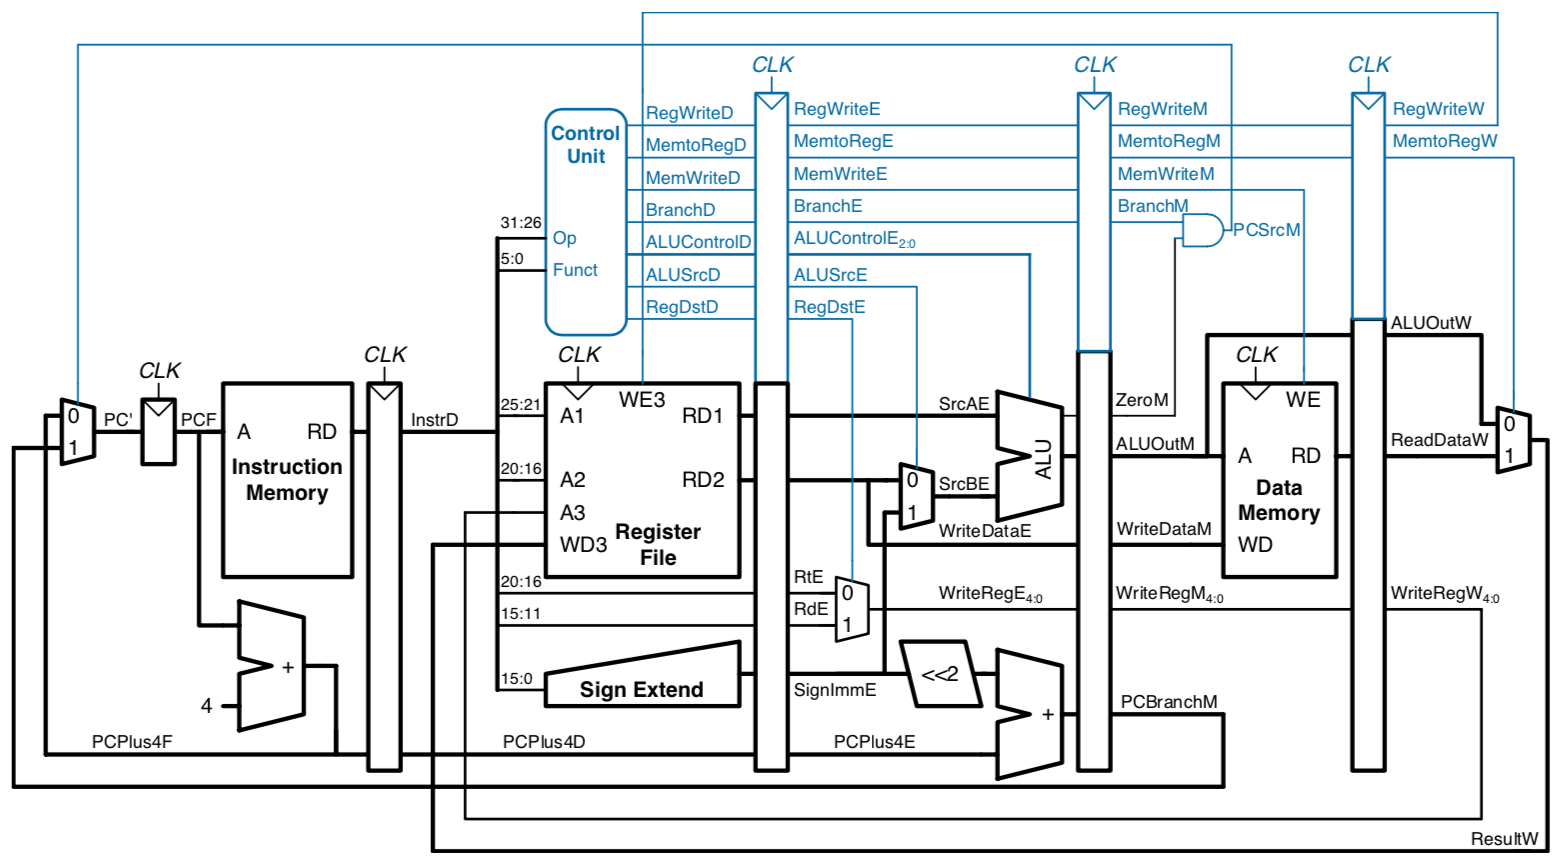
\includegraphics[width=\linewidth]{pipeline}
	\caption{Classical MIPS pipelines (without any hazard handling)}
\end{figure}
Hence, many CPUs use a strategy called pipeline which split the execution into multiple stages. Each stage stores the previous input (the output from the predecessor stage) in its register, and when the clock rises, the CPU is handling multiple instructions at different stages. The efficiency is thus largely improved.

However, lots of new problems emerge because of the pipeline:
\subsection{Control Hazards: Branch and Jump}
Just consider the CPU shown in Figure 4.1. Without pipeline, a branch instruction triggers the branching in the single cycle and setup the new PC value within the same cycle; the next instruction to execute will always be correct. However, in the pipeline model, if the branch condition fails, everything works fine; nevertheless, when the branch condition checks and the instruction reaches the Write-Back stage, there will be three invalid instructions already accumulated in the pipeline. We must find a way to flush those invalid ones.

This is actually easy, we just check the branch signal; if the branch target is set, we send a signal to all four modules before Write-Back and ask them to clear their instructions. \textbf{Notice that the memory writing should be stopped immediately while the register writing should be allowed}, because there are jumping instructions like \mintinline{asm}{jal} that will store the current PC value into a register and this operation is always valid as it arrives at the Write-Back part at the same time of the branch target.

In most CPUs, the branch cost can be further reduced by apply branch prediction and moving branching checking into an earlier stage. Here, we are not going to care about these strategies and just handle the control hazards with stalling.

\subsection{Data Hazards}
There are several kinds of data hazards:
\begin{enumerate}
\item Consecutive arithmetic operations with data dependency:
\begin{minted}[linenos]{asm}
addi $a0, $a0, 1
addi $a0, $a0, 1
addi $a0, $a0, 1
\end{minted}
Notice that when the second/third instruction reaches the Arithmetic Module, the first/second instruction is at the Memory Part/Write-Back Part; which means the write-back operation is not applied. Hence, we must figure out a way to forward the result stored in Memory Part/Write-Back Part to Arithmetic Module in advance.
\item Arithmetic Operation followed by SW:
\begin{minted}[linenos]{asm}
addi $a0, $a0, 1
sw   $a0, -4($sp)
\end{minted}
In the SW case, the value of register a0 is not ready. We can simplify the handling by moving determination of write value into Arithmetic Part. Hence, using the strategy of forwarding, we can also handle this problem.

\item LW followed by Arithmetic Operation
\begin{minted}[linenos]{asm}
lw   $t0, 0($sp)
addi $t0, $t0, 1
\end{minted}
In the pipeline shown in Figure 4.1, the load value will not be ready even with forwarding. In this case, we must stall the pipeline: keep the PC value, the state of Decode Module and the Arithmetic Module unchanged (but accepting register write-back) and insert a NOP state into memory module for the next cycle while handling the current operation of loading. Therefore, in the next cycle, the second instruction is still at the Arithmetic Module while the load result reaches the Write-Back Part which makes it possible to be forwarded to ALU. 
\end{enumerate}

\subsection{Special Changes}
We made several special changes to make life easier: 
\begin{enumerate}
	\item Because we are using the BRAM structure, which means that there is one cycle delay before we can get the real data, we need to forward the ALU results to the Memory Module in the same cycle so that in the next cycle the Memory Output is exactly what the instruction in the Memory Module requires.
	\begin{minted}[linenos]{asm}
j    SOME_PLACE
sw   $zero, 4($sp)
sw   $zero, 4($sp)
	\end{minted}
	Previously, when the branch target reaches Write-Back Part, the Memory Operation hasn't taken place; however, in our case, the stall caused by branching will only prevent the second Memory Operation after branching; we need to also check the branching before we want to write something into the memory. Fortunately, this is always available since, when the instruction right after branching arrives ALU, the branching instruction is exactly at the Memory Part, we can simply check whether the branching target is set or not.
	\item There is no need to care about the Load Data Hazards as we will also forward the data together with the memory fetching result. (Thanks to BRAM delay, the extra cost is little)
\end{enumerate}
\section{Implementation}
\subsection{Instruction Module}
\subsubsection{Instruction Set}
We will only implement very a small set of MIPS instructions. Let's first write some functions to help us decode the instruction:
\begin{minted}{haskell}

-- | The Format of MIPS Instructions
data Format            
  = NoType             -- ^ NoType (Specialized for NOP Instruction)
  | RType              -- ^ R-Type Instruction Format
      (BitVector 6)    -- ^ Operation Code
      (BitVector 5)    -- ^ Register S
      (BitVector 5)    -- ^ Register T
      (BitVector 5)    -- ^ Register D
      (BitVector 5)    -- ^ Extra Infomation for Shifting Amount
      (BitVector 6)    -- ^ Function Code
  | IType              -- ^ I-Type Instruction Format
      (BitVector 6)    -- ^ Operation Code
      (BitVector 5)    -- ^ Register S
      (BitVector 5)    -- ^ Register T
      (BitVector 16)   -- ^ Immediate Value
  | JType              -- ^ J-Type Instruction Format 
      (BitVector 6)    -- ^ Operation Code
      (BitVector 26)   -- ^ Jump Target
  deriving Show
\end{minted}
We will first recognize the instruction format and then transform it into each recognized instruction.
\begin{minted}{haskell}
decodeFormat :: BitVector 32 -> Format
decodeFormat 0 = NoType
decodeFormat vec =
    let opcode = slice d31 d26 vec
    in case opcode of
       0 ->
           pure RType 
               <*> (slice d31 d26)
               <*> (slice d25 d21) 
               <*> (slice d20 d16) 
               <*> (slice d15 d11) 
               <*> (slice d10 d6) 
               <*> (slice d5 d0) 
                $  vec
      code | code == 0b000010 || code == 0b000011 ->
           pure JType 
               <*> (slice d31 d26) 
               <*> (slice d25 d0) 
                $ vec
      _ ->
           pure IType 
               <*> (slice d31 d26) 
               <*> (slice d25 d21) 
               <*> (slice d20 d16) 
               <*> (slice d15 d0) 
                $  vec
\end{minted}
The format decode is trivial:
\begin{itemize}
	\item An all-zero instruction is a NOP;
	\item Otherwise, instructions with 0 opcode will be dispatched into R-Format;
	\item Instructions with special jumping opcode will be dispatched into J-Format;
	\item Other instructions are in the I-Format
\end{itemize}
After format is determined, we can then transform instructions into our inner forms:

\begin{minted}{haskell}
type Register = Unsigned 5
data Instruction
    = NOP
    | ADD Register Register Register
    | ADDI Register Register (Signed 16)
    | ADDU Register Register Register
    | ADDIU Register Register (Unsigned 16)
    | SUB Register Register Register
    | SUBU Register Register Register
    | AND Register Register Register
    | ANDI Register Register (BitVector 16)
    | NOR Register Register Register
    | OR Register Register Register
    | ORI Register Register (BitVector 16)
    | XOR Register Register Register
    | XORI Register Register (BitVector 16)
    | BEQ Register Register (Signed 16)
    | BNE Register Register (Signed 16)
    | SLT Register Register Register
    | SLTI Register Register (Signed 16)
    | SLTU Register Register Register
    | SLTIU Register Register (Unsigned 16)
    | LW Register Register (Signed 16)
    | SW Register Register (Signed 16)
    | SLL Register Register (Unsigned 5)
    | SRL Register Register (Unsigned 5)
    | SRA Register Register (Unsigned 5)
    | SLLV Register Register Register
    | SRLV Register Register Register
    | SRAV Register Register Register
    | J (Unsigned 26)
    | JAL (Unsigned 26)
    | JR (Unsigned 5)
    deriving Show
    deriving Generic
    deriving NFDataX
\end{minted}
We do not provide the function \mint{haskell}{decodeTyped :: Format -> Instruction} here as it should be easy to write and just require some repeated works to recognize the instruction based on the opcode and the function code.

Just mention a small trick: to reduce the repeated code, you can use the Applicative property of Readers):
\begin{minted}{haskell}
t1 (x, _, _) = x
t2 (_, y, _) = y
t3 (_, _, z) = z
makeType func = pure func <*> unpack . t1 <*> unpack . t2 <*> unpack . t3
-- then you can just use something like:
case fn of
    0b100000 -> (makeType ADD) (rs, rt, rd)
    0b100001 -> (makeType ADDU) (rs, rt, rd)
    0b100100 -> (makeType AND) (rs, rt, rd)
    -- more cases ...
\end{minted}
However, please notice that for most R instructions, we will keep the format as \mintinline{haskell}{ADD rs rt rd}, but for those shift related operations, the format will be \mintinline{haskell}{SLL rd rt sa}; those I instructions adapts the format of \mintinline{haskell}{ADDI rs rt imm}.
\subsubsection{The Instruction RAM}
We will use BRAM to implement the instruction memory space. The memory itself is quite simple, we just use the  \mintinline{haskell}{blockRamFile} function to achieve the goal
\begin{minted}[breaklines]{haskell}
instrRAM' 
  ::  HiddenClockResetEnable dom
  => Signal dom MemAddr
  -> Signal dom (BitVector 32)
instrRAM' = (flip $ blockRamFile d512 "instructions.bin") $ pure Nothing

instrRAM 
  :: Clock System
  -> Reset System
  -> Enable System
  -> Signal System MemAddr
  -> Signal System (BitVector 32)
instrRAM = exposeClockResetEnable instrRAM'
\end{minted}
\subsubsection{Instruction Module Interface}
Now we must think carefully of what we are going to in this module:
\begin{enumerate}
	\item We need to maintain the value of program counter, if not branching happens, we just increase it; otherwise, we set the counter to the branch target immediately.
	\item Each cycle we will need to output two things: an instruction and (PC + 1) (one plus the instruction index). As BRAM has an delay effect, the current PC in this cycle is exactly the value we want, hence we do not need to make an extra addition to the counter.
	\item When stall happens, output a NOP. As the branch target is set immediately, there is no need to keep the old PC value.
\end{enumerate}
With these ideas, we can come out the following design:
\begin{figure}[H]
	\centering
	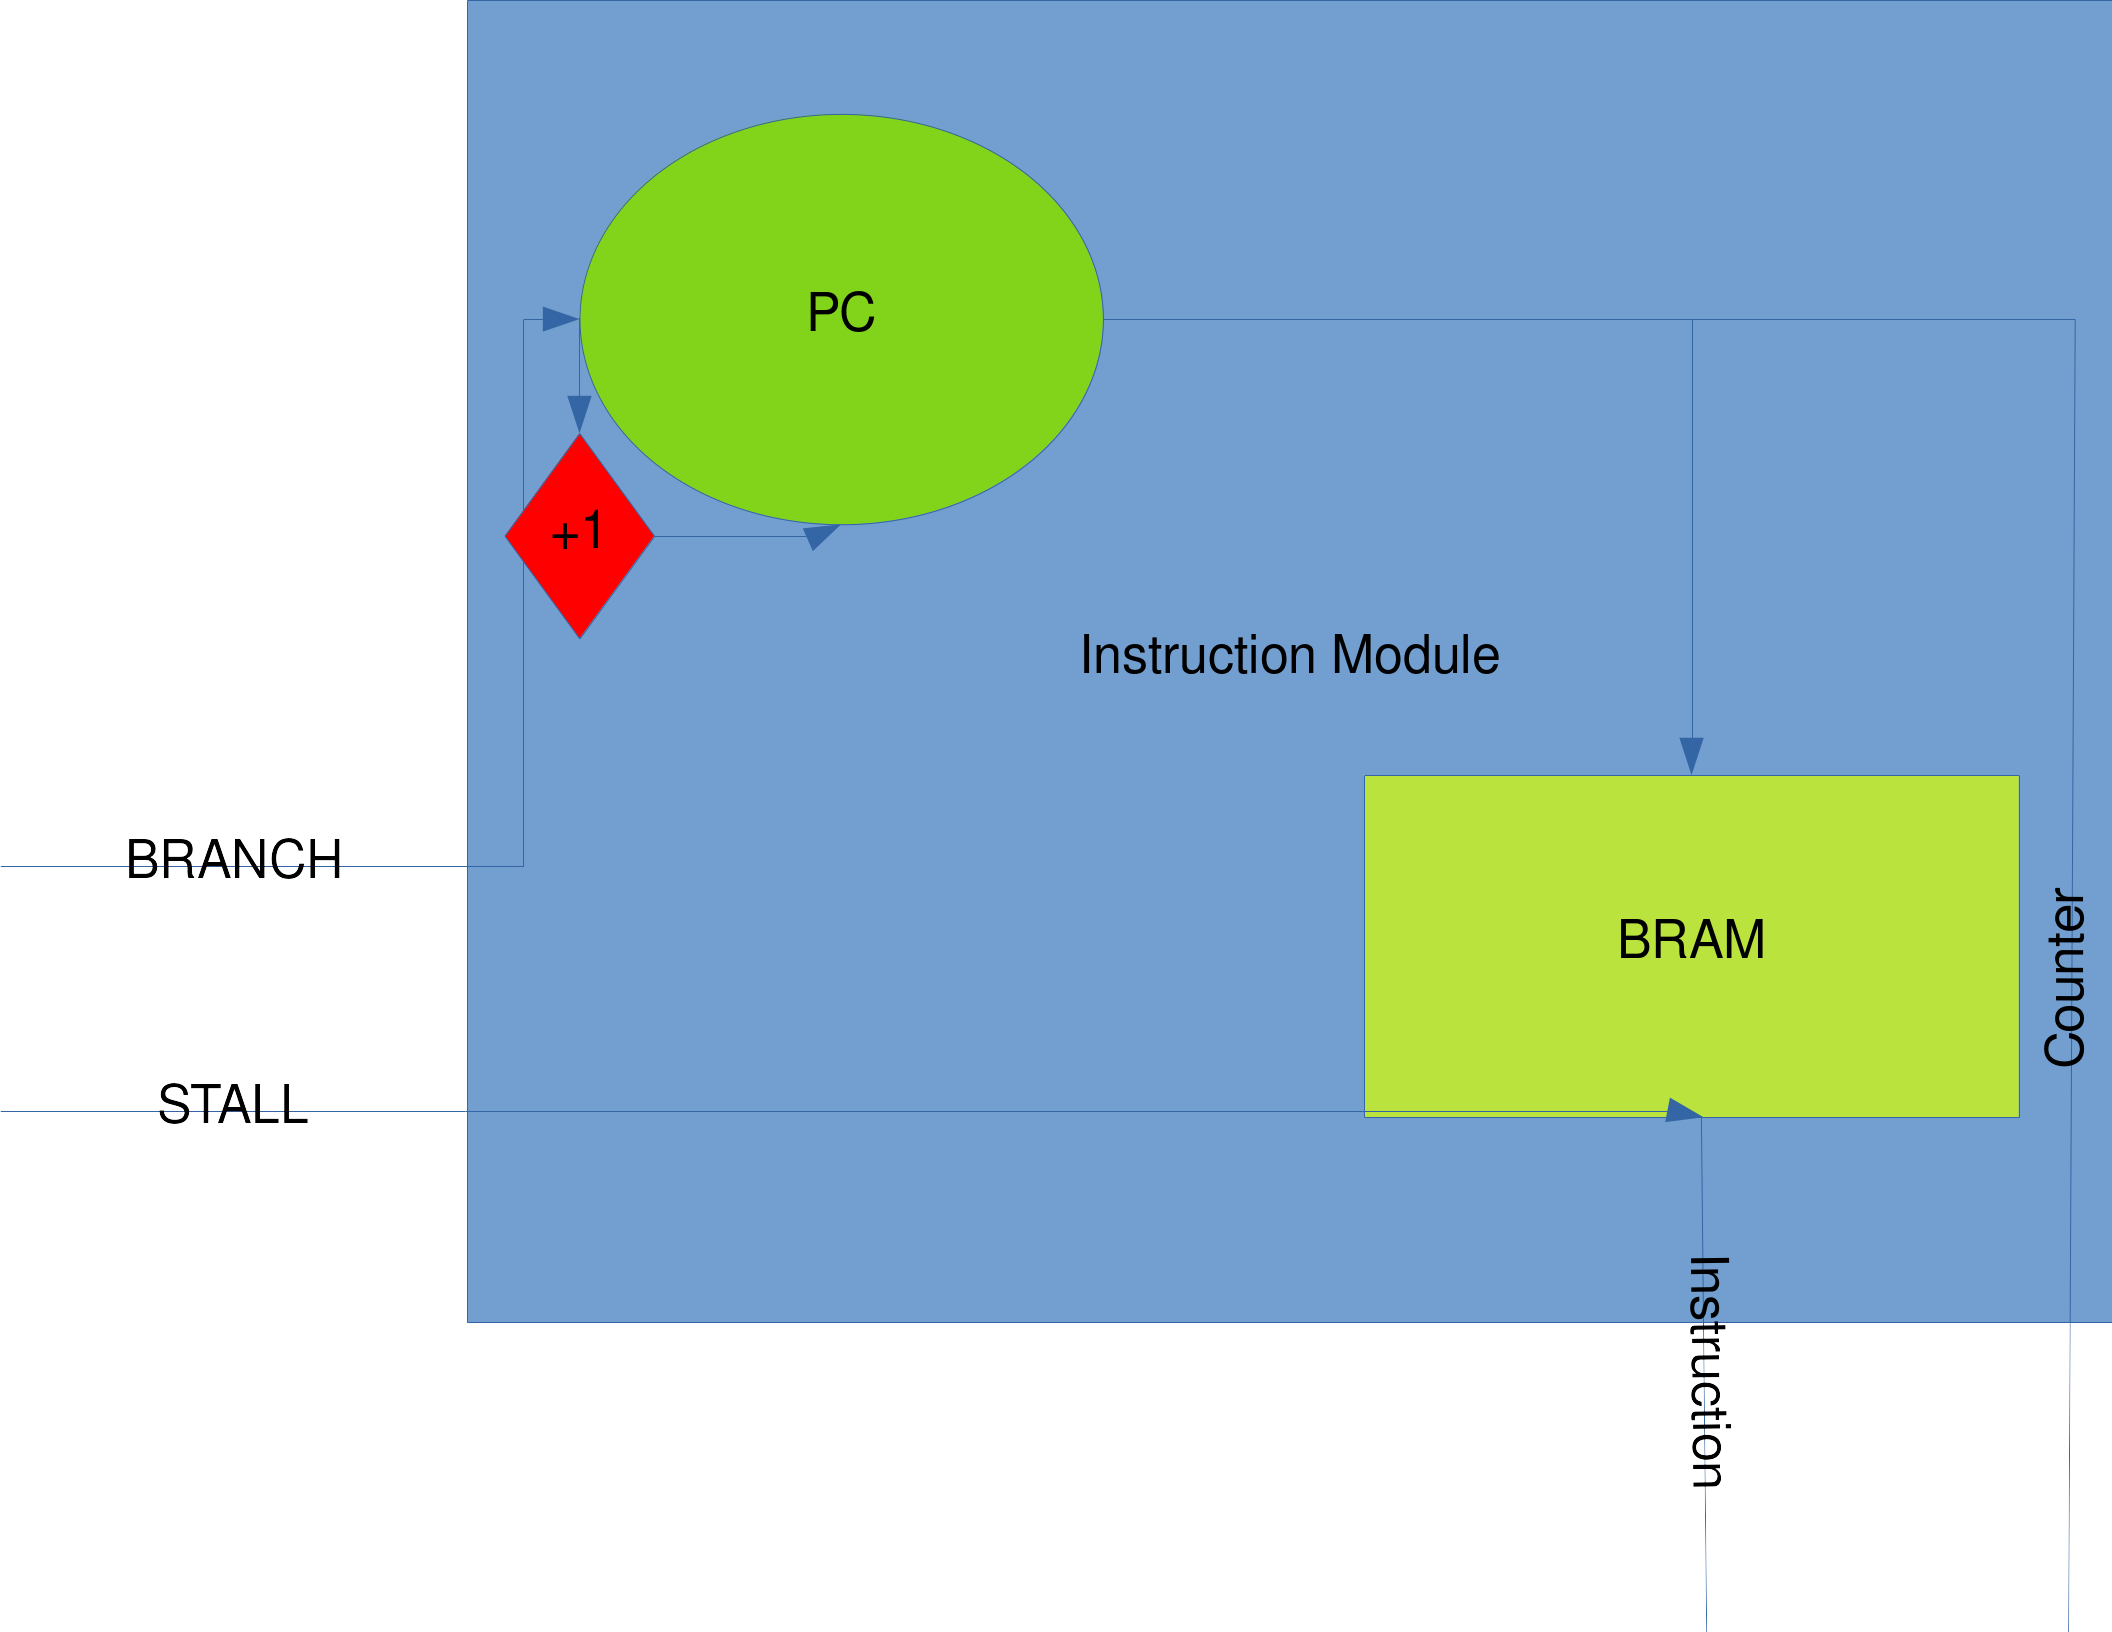
\includegraphics[width=\linewidth]{im}
	\caption{Instruction Module Diagram}
\end{figure}
Let's first maintain the PC value using a Mealy Machine:    
\begin{minted}[breaklines]{haskell}
type PCInput = Maybe (Unsigned 32)
programCounterT 
  :: Unsigned 32 
  -> PCInput
  -> (Unsigned 32, Unsigned 32)
programCounterT state (Just t) = (t + 1, t)
programCounterT state _ = (state + 1, state)

programCounter 
  :: HiddenClockResetEnable dom
  => Signal dom PCInput
  -> Signal dom (Unsigned 32)
programCounter = mealy programCounterT 0
\end{minted}
As you can see, unless the branch target is set, the PC just behaves as a monotonic counter.
\begin{minted}[breaklines, linenos]{haskell}
{-# ANN pcModule
    (Synthesize{t_name = "InstructionModule",
        t_inputs =
          [PortName "CLOCK", PortName "RESET", PortName "ENABLE", PortName "STALL", PortName "BRANCH"],
        t_output =
          PortProduct "PC" [PortName "INSTRUCTION", PortName "VALUE"]})
    #-}

pcModule 
  :: Clock System
  -> Reset System
  -> Enable System
  -> Signal System Bool
  -> Signal System (Maybe (Unsigned 32))
  -> Signal System (Instruction, (Unsigned 32))
pcModule clk rst enable stall br = bundle (instr, next)
  where
    programCounter' = (exposeClockResetEnable programCounter) clk rst enable
    next = programCounter' $ br
    ram = instrRAM clk rst enable next
    ram' = decodeTyped . decodeFormat <$> ram
    instr' op ram =
      case op of
        False -> ram
        True -> NOP
    instr = instr' <$> stall <*> ram'
\end{minted}
If you are not familiar with Haskell, just notice that $<\$>, <*>$ are the operators using the Applicative property of Signal to lift a function of \mintinline{haskell}{f :: a -> b -> c} type onto \mintinline{haskell}{f :: Signal dom a -> Signal dom b -> Signal dom c}, so that we can transform combinatorial logic into a sequential form.
The data flow is simple:
\begin{enumerate}
	\item Get the current counter with branch flag
	\item Get the memory output and set the next address to fetch
	\item Decode the output
	\item Check the stall condition and output the instruction and PC value
\end{enumerate}
Now we can happily generate the Verilog code for this module, try it!

\subsection{Decode Module}
\subsubsection{Register File}
Decode Module contains the Register File which is in charge of maintaining the register value. Let us first take a look at this part.
As the logic relation is little bit complicated, we can use State Monad to construct the state machine for the Register File.
\begin{minted}[breaklines, linenos]{haskell}
type Reg = BitVector 32

type RegNo = Unsigned 5

registerFileS 
  :: ( RegNo -- rs
     , RegNo -- rt
     , Maybe (RegNo, Reg) -- write register
     )
  -> State (Vec 32 Reg) (Reg, Reg)
registerFileS (reg0, reg1, writePair) = do
    regs <- get
    let res0 = regs !! reg0
        res1 = regs !! reg1
        newS = case writePair of
            Nothing -> regs
            Just (a, b) -> 
                if a /= 0
                then replace a b regs
                else regs
    put newS
    return (res0, res1)

{-# ANN registerFile
    (Synthesize
      { t_name = "RegisterFile"
      , t_inputs =
        [ PortName "CLOCK"
        , PortName "RESET"
        , PortName "ENABLE"
        , PortProduct "RF" 
          [ PortName "RS"
          , PortName "RT"
          , PortName "WRITE"
          ]
        ]
      , t_output = 
        PortProduct "RF" 
          [ PortName "RSV"
          , PortName "RTV"
          ]
      }
    )
#-}

registerFile 
  :: Clock System
  -> Reset System
  -> Enable System
  -> Signal System (RegNo, RegNo, Maybe (RegNo, Reg))
  -> Signal System (Reg, Reg)
registerFile = exposeClockResetEnable $ asStateM registerFileS (replicate d32 0)
\end{minted}
The Register File takes three input: two register indices to fetch and one register write serial consists of register number and target value. The output the values of the required registers.

\subsubsection{Control Unit}
Now comes one of the most tedious part of the entire CPU, the Control Unit. It extract the information from the instruction and separate them for further execution.

The extraction is not stateful, to reduce the complexity, we can argue this part in the combinatorial form and lift it later. 

Here we are going to define lots of data format for later uses:
 
\begin{itemize}
	\item \mintinline{haskell}{MemoryOperation}: this data tags the operation on the RAM: none, read or write:
	\begin{minted}[breaklines]{haskell}
data MemoryOperation
  = MemNone
  | MemLoad
  | MemWrite
deriving (Generic)
deriving (NFDataX)
deriving (Show)
	\end{minted}
	\item \mintinline{haskell}{BranchFlag}: Four types: no-branching, branch-on-equal, branch-on-different, jump; because conditional branching uses up two operands, we need additional field to carry the branching difference.
\begin{minted}[breaklines]{haskell}
data BranchFlag
  = NoBranch
  | BranchEQ (BitVector 32)
  | BranchNE (BitVector 32)
  | Jump
  deriving (Generic)
  deriving (NFDataX)
	\end{minted}
  \item \mintinline{haskell}{ALUOperation}: Defines the ALU Operations, those add, sub, set, right shift operations are accompanied with an extra bit to tag whether the data is signed or not.
\begin{minted}[breaklines]{haskell}
data ALUOperation
  = ALUAdd Bool
  | ALUSub Bool
  | ALUAnd
  | ALUNor
  | ALUOr
  | ALUXor
  | ALUSet Bool
  | ALUShiftL
  | ALUShiftR Bool
  | ALUNone
deriving (Generic)
deriving (NFDataX)
	\end{minted}
\end{itemize}
Now, we can write some functions to dispatch these flags. First, we can check whether there is a need of writing register. The correct register to write may vary with different instructions. One special case is the JAL instruction, which requires the update of register ra.
\begin{minted}[breaklines]{haskell}
writeRegister 
  :: HiddenClockResetEnable dom
  => Signal dom Instruction
  -> Signal dom (Maybe (Unsigned 5))
writeRegister = fmap writeRegister'
  where
    writeRegister' inst =
      case inst of
        ADD   _  _  rd -> Just rd
        ADDI  _  rt _  -> Just rt
        ADDU  _  _  rd -> Just rd
        ADDIU _  rt _  -> Just rt
        SUB   _  _  rd -> Just rd
        SUBU  _  _  rd -> Just rd
        AND   _  _  rd -> Just rd
        ANDI  _  rt _  -> Just rt
        NOR   _  _  rd -> Just rd
        OR    _  _  rd -> Just rd
        ORI   _  rt _  -> Just rt
        XOR   _  _  rd -> Just rd
        XORI  _  rt _  -> Just rt
        SLT   _  _  rd -> Just rd
        SLTI  _  rt _  -> Just rt
        SLTU  _  _  rd -> Just rd
        SLTIU _  rt _  -> Just rt
        SLL   rd _  _  -> Just rd
        SRL   rd _  _  -> Just rd
        SRA   rd _  _  -> Just rd
        SLLV  _  _  rd -> Just rd
        SRLV  _  _  rd -> Just rd
        SRAV  _  _  rd -> Just rd
        LW    _  rt _  -> Just rt
        JAL   _        -> Just 31
        _              -> Nothing
\end{minted}
Then, we can also check the requirement of memory operation, branching and immediate value. Here we must pay attention to the order of extend and pack to make sure that sign information is kept correctly.
\begin{minted}[breaklines]{haskell}
memoryOperation 
  :: HiddenClockResetEnable dom
  => Signal dom Instruction
  -> Signal dom MemoryOperation
memoryOperation = fmap memoryOperation'
  where
    memoryOperation' inst =
      case inst of
        LW _ _ _ -> MemLoad
        SW _ _ _ -> MemWrite
        _        -> MemNone

branchFlag 
  :: HiddenClockResetEnable dom
  => Signal dom Instruction
  -> Signal dom BranchFlag
branchFlag = fmap branchFlag'
  where
    branchFlag' inst =
      case inst of
        BEQ _ _ x -> BranchEQ (pack $ extend x)
        BNE _ _ x -> BranchNE (pack $ extend x)
        JR  _     -> Jump
        J   _     -> Jump
        JAL _     -> Jump
        _         -> NoBranch

immediateValue 
  :: HiddenClockResetEnable dom
  => Signal dom Instruction
  -> Signal dom (Maybe (BitVector 32))
immediateValue = fmap immediateValue'
  where
    immediateValue' inst =
      case inst of
        ADDI  _ _ x -> Just (pack $ extend x)
        ADDIU _ _ x -> Just (pack $ extend x)
        ANDI  _ _ x -> Just (extend x)
        ORI   _ _ x -> Just (extend x)
        XORI  _ _ x -> Just (extend x)
        SLTI  _ _ x -> Just (pack $ extend x)
        SLTIU _ _ x -> Just (pack $ extend x)
        LW    _ _ x -> Just (pack $ extend x)
        SW    _ _ x -> Just (pack $ extend x)
        SLL   _ _ x -> Just (pack $ extend x)
        SRL   _ _ x -> Just (pack $ extend x)
        SRA   _ _ x -> Just (pack $ extend x)
        JAL   x     -> Just (pack $ extend x)
        J     x     -> Just (pack $ extend x)
        _           -> Nothing
\end{minted}
The next part is little bit tricky: dispatching the ALU operation. Basic arithmetic operation can be dispatched directly. Notwithstanding, there are some special cases. For example, BEQ and BNE are dispatched to XOR because we want to use the zero flag of the xor result to check whether two operands are equal. Those memory related operations are dispatched to addition, because we want to add up the immediate value and the value of RS to get the target address. As for jump operations, we will pass the jump target via immediate value so we just use the OR operation (another operand will be 0).  
\begin{minted}[breaklines]{haskell}
dispatch 
  :: HiddenClockResetEnable dom
  => Signal dom Instruction
  -> Signal dom ALUOperation
dispatch = fmap dispatch'
  where
    dispatch' inst =
      case inst of
        ADD   _ _ _ -> ALUAdd True
        ADDI  _ _ _ -> ALUAdd True
        ADDU  _ _ _ -> ALUAdd False
        ADDIU _ _ _ -> ALUAdd False
        SUB   _ _ _ -> ALUSub True
        SUBU  _ _ _ -> ALUSub False
        AND   _ _ _ -> ALUAnd
        ANDI  _ _ _ -> ALUAnd
        NOR   _ _ _ -> ALUNor
        OR    _ _ _ -> ALUOr
        ORI   _ _ _ -> ALUOr
        XOR   _ _ _ -> ALUXor
        XORI  _ _ _ -> ALUXor
        BEQ   _ _ _ -> ALUXor
        BNE   _ _ _ -> ALUXor
        SLT   _ _ _ -> ALUSet True
        SLTI  _ _ _ -> ALUSet True
        SLTU  _ _ _ -> ALUSet False
        SLTIU _ _ _ -> ALUSet False
        LW    _ _ _ -> ALUAdd True
        SW    _ _ _ -> ALUAdd True
        SLL   _ _ _ -> ALUShiftL
        SLLV  _ _ _ -> ALUShiftL
        SRL   _ _ _ -> ALUShiftR False
        SRLV  _ _ _ -> ALUShiftR False
        SRA   _ _ _ -> ALUShiftR True
        SRAV  _ _ _ -> ALUShiftR False
        JR    _     -> ALUOr
        J     _     -> ALUOr
        JAL   _     -> ALUOr
        _           -> ALUNone
\end{minted}

Finally, we can finish the Control Unit interface:

\begin{minted}[breaklines]{haskell}
{-# ANN controlUnit
  ( Synthesize
    { t_name = "ControlUnit"
    , t_inputs =
        [ PortName "CLOCK"
        , PortName "RESET"
        , PortName "ENABLE"
        , PortName "Instruction"
        ]
    , t_output =
        PortProduct "CTL"
          [ PortName "WRITE"
          , PortName "MEM"
          , PortName "BRANCH_FLAG"
          , PortName "ALU"
          , PortName "IMM"
          ]
    }
  )
#-}

controlUnit 
  :: Clock System
  -> Reset System
  -> Enable System
  -> Signal System Instruction                 -- instruction
  -> ( Signal System (Maybe (Unsigned 5))      -- write register
     , Signal System MemoryOperation           -- memory
     , Signal System BranchFlag                -- branch flag
     , Signal System ALUOperation              -- ALU control
     , Signal System (Maybe (BitVector 32))    -- immediate value
     )
controlUnit =
  exposeClockResetEnable $
    pure (,,,,) 
      <*> writeRegister 
      <*> memoryOperation 
      <*> branchFlag 
      <*> dispatch 
      <*> immediateValue
\end{minted}
As you can see, we just collect all the parts together, making no special change.
\subsubsection{Decode Module Interface}
Eventually, we complete our design of the Control Unit and get back to the Decode Module. Unfortunately, there is still one more thing to do: to decide registers to fetch. This is described in the following function:
\begin{minted}[breaklines]{haskell}
registerPair 
  :: HiddenClockResetEnable dom
  => Signal dom Instruction
  -> Signal dom (RegNo, RegNo)
registerPair = fmap registerPair'
  where
    registerPair' inst =
      case inst of
        ADD   x y _ -> (x, y)
        ADDI  x _ _ -> (x, 0)
        ADDU  x y _ -> (x, y)
        ADDIU x _ _ -> (x, 0)
        SUB   x y _ -> (x, y)
        SUBU  x y _ -> (x, y)
        AND   x y _ -> (x, y)
        ANDI  x _ _ -> (x, 0)
        NOR   x y _ -> (x, y)
        OR    x y _ -> (x, y)
        ORI   x _ _ -> (x, 0)
        XOR   x y _ -> (x, y)
        XORI  x _ _ -> (x, 0)
        BEQ   x y _ -> (x, y)
        BNE   x y _ -> (x, y)
        SLT   x y _ -> (x, y)
        SLTI  x _ _ -> (x, 0)
        SLTU  x y _ -> (x, y)
        SLTIU x _ _ -> (x, 0)
        LW    x _ _ -> (x, 0)
        SW    x y _ -> (x, y)
        SLL   _ x _ -> (x, 0)
        SRL   _ x _ -> (x, 0)
        SRA   _ x _ -> (x, 0)
        SLLV  x y _ -> (y, x)
        SRLV  x y _ -> (y, x)
        SRAV  x y _ -> (y, x)
        NOP         -> (0, 0)
        J     _     -> (0, 0)
        JAL   _     -> (0, 0)
        JR    x     -> (x, 0)
\end{minted}
For those who requires immediate values, we just set the second register to zero and it will not be used. The jump operations' first register will also be set to zero to make sure that OR operation will preserve the immediate value.
Next, let us write a function to handle the state transition of the decode module: at the rising edge of the clock, this module will store the output as the new state and handle the decoding of the previous state.
\begin{minted}[breaklines]{haskell}
type DecodeModuleState = (Instruction, Unsigned 32)

decodeModuleState 
  :: (Instruction, Unsigned 32, Bool)
  -> State DecodeModuleState DecodeModuleState
decodeModuleState (inst, pc, stall) = do
  case stall of
    False -> do
      state <- get
      put (inst, pc)
      return state
    True -> do
      let res = (NOP, 0)
      put res
      return res
\end{minted}
Special cases occur when the stall flag is set; it will then flush the output and state by setting the instruction to NOP.
\begin{minted}{haskell}
{-# ANN decodeModule
    ( Synthesize
      { t_name = "DecodeModule"
      , t_inputs =
          [ PortName "CLOCK"
          , PortName "RESET"
          , PortName "ENABLE"
          , PortName "WRITE_REG"
          , PortName "STALL"
          , PortName "INSTRUCTION"
          , PortName "COUNTER"
          ]
      , t_output =
          PortProduct "DM"
            [ PortName "WRITE"
            , PortName "MEM"
            , PortName "BRANCH_FLAG"
            , PortName "ALU"
            , PortName "IMM"
            , PortName "RS"
            , PortName "RSV"
            , PortName "RT"
            , PortName "RTV"
            , PortName "COUNTER"
            ]
       }
    )
#-}
decodeModule 
  :: Clock System
  -> Reset System
  -> Enable System
  -> Signal System ( Maybe (RegNo, Reg) )   -- write data
  -> Signal System Bool                     -- stall
  -> Signal System Instruction              -- instruction
  -> Signal System ( Unsigned 32 )          -- counter
  -> Signal System ( Maybe ( Unsigned 5 )   -- write register
                   , MemoryOperation        -- memory
                   , BranchFlag             -- branch flag
                   , ALUOperation           -- ALU control
                   , Maybe ( BitVector 32 ) -- immediate value
                   , RegNo                  -- rs
                   , BitVector 32           -- rs value
                   , RegNo                  -- rd
                   , BitVector 32           -- rd value
                   , Unsigned 32            -- output counter
                   )
decodeModule clk rst enable wdata stall inst counter =
  let stateMachine    =
        exposeClockResetEnable $ asStateM decodeModuleState (NOP, 0)
      (rinst, pc)     =
        unbundle (stateMachine clk rst enable $ bundle (inst, counter, stall))
      regDecoder      = 
        exposeClockResetEnable registerPair
      (rs, rt)        = 
        unbundle $ regDecoder clk rst enable rinst
      (w, m, b, a, i) = 
        controlUnit clk rst enable rinst
      (rsv, rtv)      =
        unbundle (registerFile clk rst enable $ bundle (rs, rt, wdata))
  in  bundle (w, m, b, a, i, rs, rsv, rt, rtv, pc)
\end{minted}
Finally, we come up with the interface of the whole module. On clock rising, the module will first handle the state transition and get the instruction from its own register. Based on the instruction, it decides the register to read and generate the output in the control unit. One special part is that the register writing information is not from the state register and the module will handle the external write request at the same cycle. The read and write information are set to the register file. The numbers of the register operands will also be passed to the next module, because they are useful to decide the forwarding information in ALU. On stalling, this module will just behaves as if the current instruction is NOP, but the writing requests are handled correctly.
\begin{figure}[H]
	\centering
	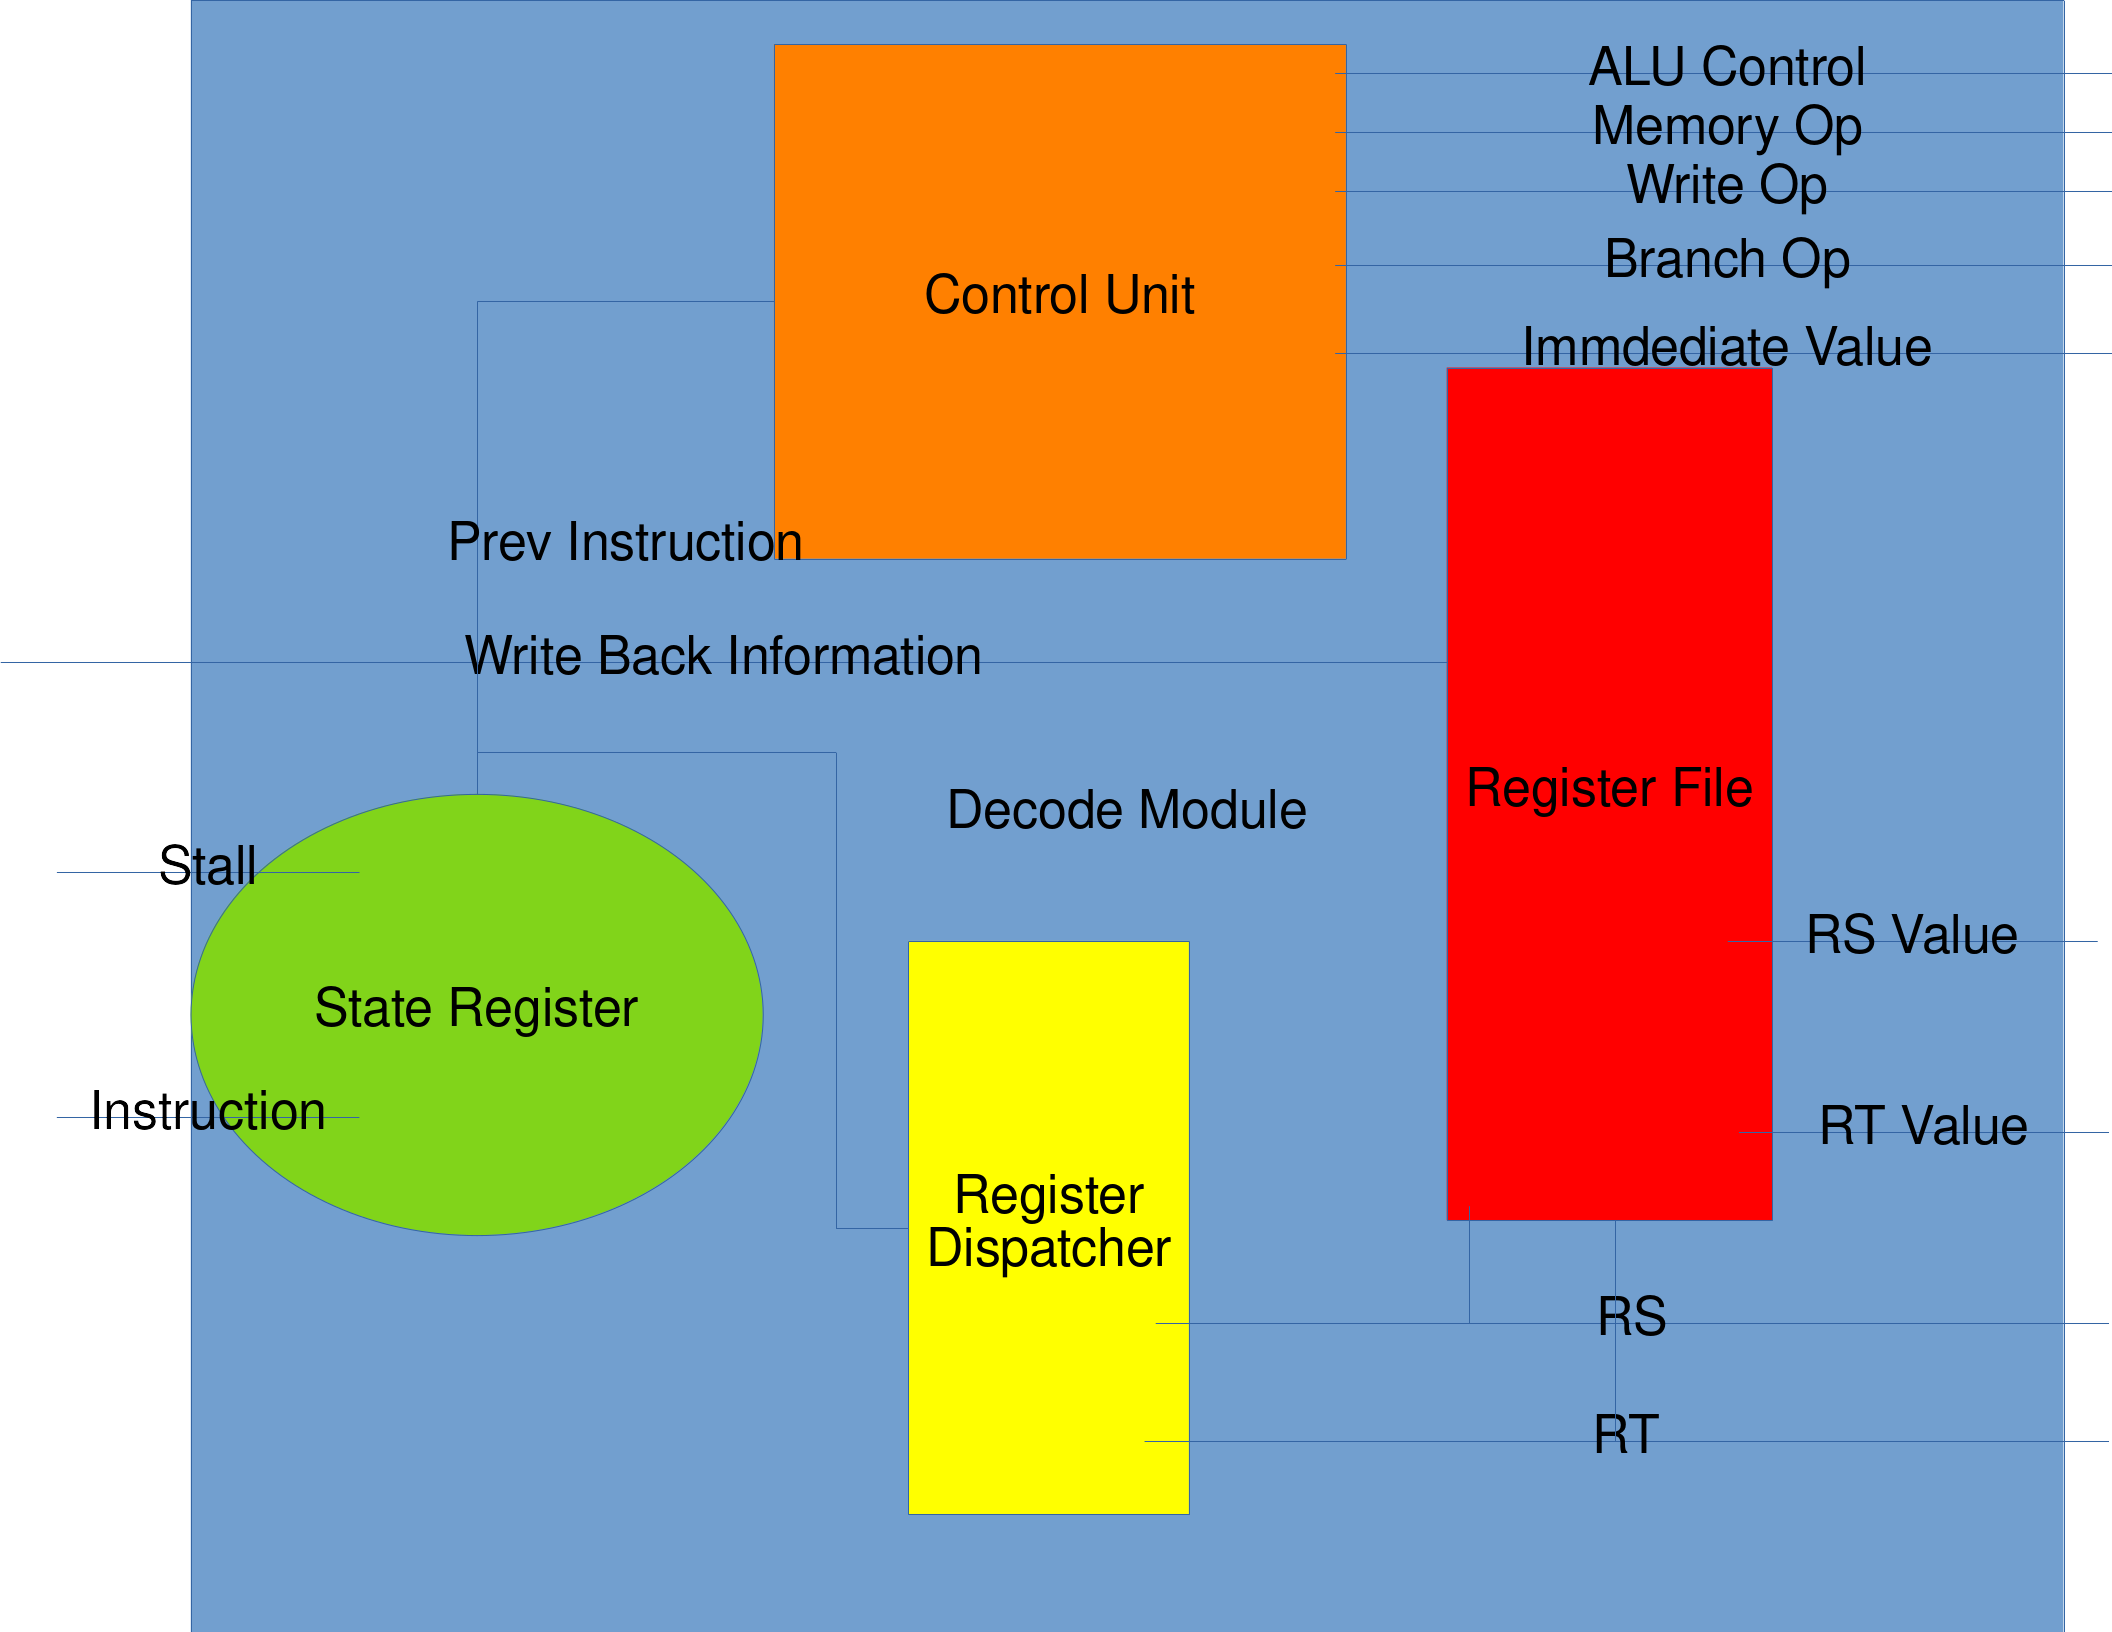
\includegraphics[width=\linewidth]{dm}
	\caption{Decode Module Diagram)}
\end{figure}
\subsection{Arithmetic Module}
Arithmetic Module is in charge of calculations. It will also check the branching condition and determine the target. Memory Operation cannot live without this module either, as the memory address is decided in this part.
\subsubsection{Data Types}
In order to make life easier, let us first define some data types:
\begin{itemize}
\item \mintinline{haskell}{MemoryOperation'}: This will be one of the output of this module. Previously, we have already defined \mintinline{haskell}{MemoryOperation}. This new data type is almost the same, but the write operation carries its writing value now as the value is now ready after arithmetic operations.
\begin{minted}{haskell}
data MemoryOperation'
  = MemNone'
  | MemLoad'
  | MemWrite' (BitVector 32)
deriving (Generic)
deriving (NFDataX)
deriving (Show)
\end{minted}
\item  \mintinline{haskell}{ALUState}: just the same as the output product of the Decode Module.
\item  \mintinline{haskell}{ALUOutput}: a product type of the output of this module
\begin{minted}{haskell}
type ALUOutput
  = ( Maybe (Unsigned 5)  -- write register
    , MemoryOperation'    -- memory
    , BitVector 32        -- ALU result
    , Maybe (Unsigned 32) -- branch target
    )
\end{minted}
\end{itemize}
\subsubsection{ALU}
ALU is a combinatorial circuit within the CPU that handles most of the arithmetic works. Here, our ALU follows the control command sent from the Control Unit and apply the target operations on its operands. Apart from the arithmetic result, ALU will also generate some flags like zero, negative and overflow. Although only zero flag is useful for this book, we are going to implement all these flags. For additions, overflow happens if the operands has the same sign bit while the sign bit changed in the result; for subtraction, overflow happens if the operands has different sign bit while the signed bit of the result is the same as the second operand. The following functions implement the detection of overflow:
\begin{minted}{haskell}
addOverflow :: BitVector 32 -> BitVector 32 -> (BitVector 32, Bool)
addOverflow a b =
  let c = a + b
  in (c, (a ! 31) == (b ! 31) && (a ! 31) /= (c ! 31))

subOverflow :: BitVector 32 -> BitVector 32 -> (BitVector 32, Bool)
subOverflow a b =
  let c = a - b
  in (c, (a ! 31) /= (b ! 31) && (c ! 31) == (b ! 31))
\end{minted}

The interface of ALU is described as the following:
\begin{minted}{haskell}
type ALUResult
  = ( BitVector 32 -- Arithmetic Result
    , Bool -- Overflow Result
    , Bool -- Zero Flag
    , Bool -- Negative Flag
    )

{-# ANN arithmeticUnit
    ( Synthesize
      { t_name = "ArithmeticUnit"
      , t_inputs =
          [ PortName "OPERATION"
          , PortName "OPERAND_1"
          , PortName "OPERAND_2"
          ]
      , t_output =
          PortProduct "ALU"
            [ PortName "RESULT"
            , PortName "OVERFLOW"
            , PortName "ZERO"
            , PortName "NEG"
            ]
       }
     )
#-}

arithmeticUnit :: ALUOperation -> BitVector 32 -> BitVector 32 -> ALUResult
arithmeticUnit op opr0 opr1 = (res, o, z, n)
  where
    (res, o, n) = arithmeticUnit' op
    z = res == 0
\end{minted}
The following part is the inner implementation of each operation:
\begin{enumerate}
	\item Addition and Subtraction: signed and unsigned addition change the bits in the same way, but only signed operation may overflow. 
	\begin{minted}{haskell}
arithmeticUnit' (ALUAdd flag) =
  let (res, overflow) = addOverflow opr0 opr1
  in (res, overflow && flag, bitToBool $ res ! 31)
arithmeticUnit' (ALUSub flag) =
  let (res, overflow) = subOverflow opr0 opr1
  in (res, overflow && flag, bitToBool $ res ! 31)
	\end{minted}
	\item And, Or, Xor, Nor are simple bitwise operations:
	\begin{minted}{haskell}
arithmeticUnit' ALUAnd = (opr0 .&. opr1, False, False)
arithmeticUnit' ALUNor = (complement $ opr0 .|. opr1, False, False)
arithmeticUnit' ALUOr  = (opr0 .|. opr1, False, False)
arithmeticUnit' ALUXor = (opr0 `xor` opr1, False, False) 
	\end{minted}
	\item Set-on-less-than needs to distinguish the sign information:
	\begin{minted}{haskell}
arithmeticUnit' (ALUSet flag) =
  let result =
    boolToBV $
      if flag
      then (unpack opr0 :: Signed 32)   < (unpack opr1 :: Signed 32)
      else (unpack opr0 :: Unsigned 32) < (unpack opr1 :: Unsigned 32)
  in (result, False, False)
\end{minted}
\item Shift operations can use the predefined functions in Clash but we need to check the sign information for the right shifting:
\begin{minted}{haskell}
arithmeticUnit' ALUShiftL =
  (opr0 `shiftL` (unpack $ extend opr1), False, False)
arithmeticUnit' (ALUShiftR True) =
  ( pack $ (unpack opr0 :: Signed 32) `shiftR` (unpack $ extend opr1)
  , False
  , False)
arithmeticUnit' (ALUShiftR False) =
  (opr0 `unsafeShiftR` (unpack $ extend opr1), False, False)
\end{minted}
\item Non-Operation does nothing:
\begin{minted}{haskell}
arithmeticUnit' ALUNone = (0, False, False)
\end{minted}
\end{enumerate}
\end{document}